%% Springer Nature LaTeX template (sn-jnl.cls) supplied with the submission.
\documentclass[lineno,pdflatex,sn-apa]{sn-jnl}% Math and Physical Sciences Numbered Reference Style

%%%% Standard Packages
\usepackage{graphicx}%
\usepackage{multirow}%
\usepackage{amsmath,amssymb,amsfonts}%
\usepackage{amsthm}%
\usepackage{mathrsfs}%
\usepackage[title]{appendix}%
\usepackage{xcolor}%
\usepackage{textcomp}%
\usepackage{manyfoot}%
\usepackage{booktabs}%
\usepackage{algorithm}%
\usepackage{algorithmicx}%
\usepackage{algpseudocode}%
\usepackage{listings}%
\let\orcidlogo\undefined
\usepackage{orcidlink}%
%%%%

\theoremstyle{thmstyleone}%
\newtheorem{theorem}{Theorem}%
\newtheorem{proposition}[theorem]{Proposition}%

\theoremstyle{thmstyletwo}%
\newtheorem{example}{Example}%
\newtheorem{remark}{Remark}%

\theoremstyle{thmstylethree}%
\newtheorem{definition}{Definition}%

\raggedbottom


\begin{document}



\title[Online Resource 1]{Online Resource 1: Supplementary methods and monitoring diagnostics}



\author*[1,2]{\fnm{Junjie} \sur{Zhang}\,\orcidlink{0009-0004-8821-4018}}\email{junjiezhang2024@shisu.edu.cn}

\affil*[1]{\orgdiv{Shanghai Academy of Global Governance and Area Studies}, \orgname{Shanghai International Studies University}, \orgaddress{\city{Shanghai}, \postcode{201620}, \country{China}}}

\affil[2]{\orgdiv{School of Economics and Finance}, \orgname{Shanghai International Studies University}, \orgaddress{\city{Shanghai}, \postcode{201620}, \country{China}}}


\abstract{Acquisition surrogate equations, reference units and support definitions, forward residual persistence, candidate utility diagnostics and computational verification for the sparse river nutrient monitoring assessment.}



\keywords{acquisition score; reference units; residual persistence; computational verification}



\maketitle



\section*{S1. Acquisition surrogate and pooled output state}

These equations specify the acquisition surrogate and the pooled output model, and the main comparisons use the latest residual correction described in the Materials and methods. In the mechanism tests, the assumed scoring delay replaces $d$ in the projected covariance, the effective noise and the load functional while the real return clock is unchanged, and each purchase saves the prediction that the system actually issued. The Gaussian design identities below describe the surrogate and they are not a proven error reduction of the latest residual output.

The acquisition state uses four covariates: $\log(1+Q_t/Q_*)$, its 6 h change, and annual sine and cosine terms. Historical means and standard deviations, estimated at times with finite and nonnegative observed discharge, standardise the inputs. Four fixed Gaussian frequency vectors with unit length scale produce paired cosine and sine features, each divided by $\sqrt{4}$, plus an intercept. The resulting $z_t$ therefore has nine components, following the random Fourier feature construction of Rahimi and Recht \citep{rahimi2007}. Each replay begins with zero residual information, and the feature map stays fixed throughout the year.

Let $\lambda=2^{-1/h}$, where the selected forgetting half life is $h=2160$ h. For reference qualified samples collected at $s$ and successfully returned by $t$, the residual information state is

\begin{align}
A_t &= v_0^{-1}I+\sum_{s\in\mathcal R_t} \frac{\lambda^{t-s}}{R_s}z_sz_s^{\mathsf T},\\
b_t &= \sum_{s\in\mathcal R_t} \frac{\lambda^{t-s}}{R_s}z_s[c_s-c_0(x_s)].
\end{align}

With $P_t=A_t^{-1}$ and $m_t=P_tb_t$, the hourly estimate is

\begin{equation}
\widehat c_t=\max\{0,c_0(x_t)+z_t^{\mathsf T}m_t\}.
\end{equation}

Hourly discounting retains the prior precision. Returned measurements enter through rank one updates that use their collection time features, frozen prior predictions and collection time variance proxies $R_s$, discounted by their full age since collection, and arrival time covariates never replace collection time covariates.

To let concentration values affect subsequent selection, each returned response updates the noise proxy using its prediction error at collection:

\begin{equation}
R\leftarrow\operatorname{clip}\{(1-\rho)R+ \rho(c_s-\widehat c_s)^2,\ 0.1R_0,\ 10R_0\}, \qquad \rho=0.1.
\end{equation}

Purchased samples retain their original $R_s$. Innovations combine predictor error, temporal variation and measurement error, and this rule does not separate those components. Residual correction itself is established in water quality estimation \citep{zhang2019}, while the implementation here enforces delayed availability and the declared acquisition state. Its covariance remains an uncalibrated design surrogate.

\section*{Delayed sampling value score}

A target specific variance reduction serves as the sampling heuristic, consistent with the general expected utility view of experimental design \citep{chaloner1995}. At a candidate time $t$, the current information state is projected to $t+d$, which discounts existing information and includes the expected information from pending samples scheduled to arrive by then. The covariance is $P_t^-$. Pending samples are provisionally treated as usable, their failures are revealed only at arrival, and no pending concentration value is used.

Future discharge is represented by persistence of the currently available discharge. Future calendar features are known, and lag changes use only observed history together with that persistence assumption. For the selected 72 h window that begins at response arrival, define

\begin{align}
v_t &= \sum_{u=t+d}^{t+d+H_t-1} 0.001(3600)\widetilde Q_u\widetilde z_u,\\
H_t &= \min(72,T-t-d).
\end{align}

with $H_t$ truncated below at zero. The score is

\begin{equation}
S_t=\frac{(v_t^{\mathsf T}P_t^-z_t)^2} {R_t/\lambda^d+z_t^{\mathsf T}P_t^-z_t}.
\end{equation}

This is the rank one variance reduction of a linear residual load functional under the Gaussian surrogate, expressed in squared load units. It holds the projected coefficient state fixed within the forecast window and it does not model future purchases, future innovations, discharge forecast errors or the effect of nonnegative prediction clipping, so it provides neither calibrated load uncertainty nor an optimality guarantee for the monitoring problem.

A fixed library of up to 96 randomly selected historical contexts supplies a relative threshold. At each decision, all library contexts are scored under the same current $P_t^-$, effective noise and remaining horizon as the candidate. Sampling is triggered when the candidate score is positive and reaches the 0.85 quantile of the library. Recomputing both candidate and reference scores avoids comparing a shrinking current covariance against a stale absolute threshold, and library membership is fixed before the target year and depends on neither target concentrations nor future target discharge.

\section*{S2. Reference units and support}

The independent raw record check uses 1 ft$^{3}$/s = 0.3048$^{3}$ m$^{3}$/s and kg N = Q(ft$^{3}$/s) $\times$ 0.3048$^{3}$ $\times$ 900 s $\times$ c(mg N/L) $\times$ 1000 L/m$^{3}$ $\times$ 10$^{-6}$ kg/mg. At station 02035000 on 1 January 2025 at 00:00 UTC, Q = 7350 ft$^{3}$/s and c = 0.34 mg N/L yield 208.1288224512 m$^{3}$/s, 187315.94020608 m$^{3}$ and 63.6874196700672 kg N for one quarter hour. The next two quarters have the same recorded values and the last has Q = 7320 ft$^{3}$/s, so their sum is 748499.205966336 m$^{3}$ and 254.489730028554 kg N, which matches the analysis record. This verifies absolute units independently of any cancellation in percentage errors.

Observed water coverage uses every finite and nonnegative reading on the exact quarter hour grid, weighted by 900 s, including estimated or provisional discharge and independently of concentration availability. A secondary denominator retains only qualified discharge. Neither denominator estimates runoff during absent discharge readings. Complete reference hours require the four qualified joint discharge and concentration pairs, and no concentration interpolation or annual scaling is applied. Instrument methods, inclusion and exclusion reasons and complete station year support are retained in the electronic data tables.

\section*{S3. Forward residuals and process timing}

For each station year the seed 41 historical calibration forest is reconstructed from earlier years and predicts all hours of the latest eligible historical calibration year, and its original error audit of up to 4000 observations was reproduced in all 43 included contexts. Historical lag correlations require exactly lagged qualified pairs and a qualified intervening hour at every step, and endpoint only pairs are reported separately. In sample historical predictions do not enter these persistence diagnostics. The historical discharge scaling of the earlier experiment is retained, which makes this forward concentration withholding rather than fully nested scaling, and target minus history residual changes combine environmental variation, model refitting and support selection.

Onset based elapsed transport fractions use eligible events and complete reference hours. Event medians give each event equal weight, and load weighted fractions divide summed early mass by summed event mass. Actual policy first arrival fractions instead locate the first successful return inside the event interval, including samples collected before onset. When no result returns during the event the fraction is defined as one and a separate no arrival flag is retained, because earlier information may still influence the estimate. At a temporal budget of 96 samples, the equal station mean fraction of reference mass transported before the first usable arrival is 48.13\% for load value and 46.97\% for flow triggering, and the no arrival fractions are 22.80\% and 18.27\%. Seeds are averaged within event, events within station, and then stations with equal weight. These quantities are descriptive rather than unavoidable estimation error.

The three process cases use all 46 eligible events at a budget of 96 samples and seed 41. Selection minimises, maximises and approaches the median of the absolute relative error difference between load value and flow triggering, with ties broken by station, year and event and distinct events required. Four policy specific loads per case were checked independently against the completed replay event records, and separate marker tracks distinguish collection, usable arrival and block expiry.

\section*{S4. Candidate utility and factor comparisons}

The monthly candidate diagnostic starts from the development periodic calendar at a budget of 96 samples and seed 41. It nominates 12:00 UTC on the 15th of each month without reading future concentration, reference quality or error, and all 168 nominated times remain in the outputs with no replacement. Eligibility after nomination requires feasible spacing, no duplicate purchase, a successful virtual sample, at least 95\% common reference support in the 72 h after the 24 h arrival, and positive reference mass. Future labels serve only these evaluation screens and the error scoring. The original future calendar and the saved sample innovation weights remain fixed, and an added sample changes the latest correction until the next scheduled successful arrival. The result therefore diagnoses score alignment conditional on one additional observation rather than evaluating a new equal budget closed loop policy. Rank associations are descriptive without inferential P values, and the complete beneficial and harmful observations are supplied.

The reconstruction factorial holds each simple calendar fixed and includes every combination of three nominal half lives, two age origins and two update families on development records. Equal numerical forgetting scales do not imply equal effective responses, because the pooled model discounts information while retaining prior precision and the latest correction discounts amplitude. The declared main output is retained for all evaluation years, and station paired intervals describe the finite monitored population and are pointwise across contrasts.

\section*{S5. Computational verification}

Sixteen replay checks and five candidate checks passed. Independent calculations verified 1281 paid calendars, budget and spacing constraints, actual arrival times, common event support, 140 aggregate metric rows and 48 principal paired comparisons, with differences limited to floating point rounding. Context verification separately checked 344 historical lag summaries, 1656 actual arrival records, all twelve case policy loads and the raw unit example. The earlier implementation and its inputs and results were kept unchanged, and every comparison reported in the main text was recomputed from archived observations.

The checked runtime was Python 3.12.10 with NumPy 2.5.1, pandas 3.0.5, SciPy 1.18.0, scikit learn 1.9.0, PyArrow 25.0.0 and joblib 1.5.3. Thirty six automated tests and six diagnostic assertions passed, covering information timing, reference support, budgets, sample time updates and reconstruction boundaries. Historical context cache keys include both the context code and its replay dependency. Acquisition manifests retain station year identifiers, exact query URLs, retrieval times, checksums and response sizes, and preparation manifests connect archived responses, quality decisions, code dependencies and derived data checksums. Original responses remain versioned and read only, and a later live data download need not reproduce the archived vintage.

\begin{center}
\noindent\textbf{Table S1} Stations with qualified working records
\end{center}

\begin{center}
\footnotesize
\setlength{\tabcolsep}{2pt}
\begin{tabular}{@{}p{0.134\textwidth}p{0.546\textwidth}p{0.111\textwidth}p{0.089\textwidth}@{}}
\toprule
USGS station & Station name & State & HUC4\\
\midrule
01491000 & Choptank River Near Greensboro, Md & Maryland & 0206\\
01646500 & Potomac River Near Wash, Dc Little Falls Pump Sta & Maryland & 0207\\
02035000 & James River At Cartersville, Va & Virginia & 0208\\
03216070 & Ohio River At Ironton, Oh & Ohio & 0509\\
03290500 & Kentucky River At Lock 2 At Lockport, Ky & Kentucky & 0510\\
03339000 & Vermilion River Near Danville, Il & Illinois & 0512\\
03346500 & Embarras River At Lawrenceville, Il & Illinois & 0512\\
03353200 & Eagle Creek At Zionsville, In & Indiana & 0512\\
03374100 & White River At Hazleton, In & Indiana & 0512\\
05447500 & Green River Near Geneseo, Il & Illinois & 0709\\
05465500 & Iowa River At Wapello, Ia & Iowa & 0708\\
05482000 & Des Moines River At 2Nd Avenue At Des Moines, Ia & Iowa & 0710\\
05482300 & North Raccoon River Near Sac City, Ia & Iowa & 0710\\
05484000 & South Raccoon River At Redfield, Ia & Iowa & 0710\\
05484500 & Raccoon River At Van Meter, Ia & Iowa & 0710\\
05537980 & Des Plaines River At Route 53 At Joliet, Il & Illinois & 0712\\
05595000 & Kaskaskia River At New Athens, Il & Illinois & 0714\\
05599490 & Big Muddy River At Rte 127 At Murphysboro, Il & Illinois & 0714\\
06902000 & Grand River Near Sumner, Mo & Missouri & 1028\\
07144100 & L Arkansas R Nr Sedgwick, Ks & Kansas & 1103\\
12212050 & Fishtrap Creek At Front Street At Lynden, Wa & Washington & 1711\\
\botrule
\end{tabular}
\end{center}

The full metadata and instrument provenance inventory and each station data and event eligibility by year are supplied electronically, and presence in the working inventory does not imply inclusion in every assessment.

\begin{center}
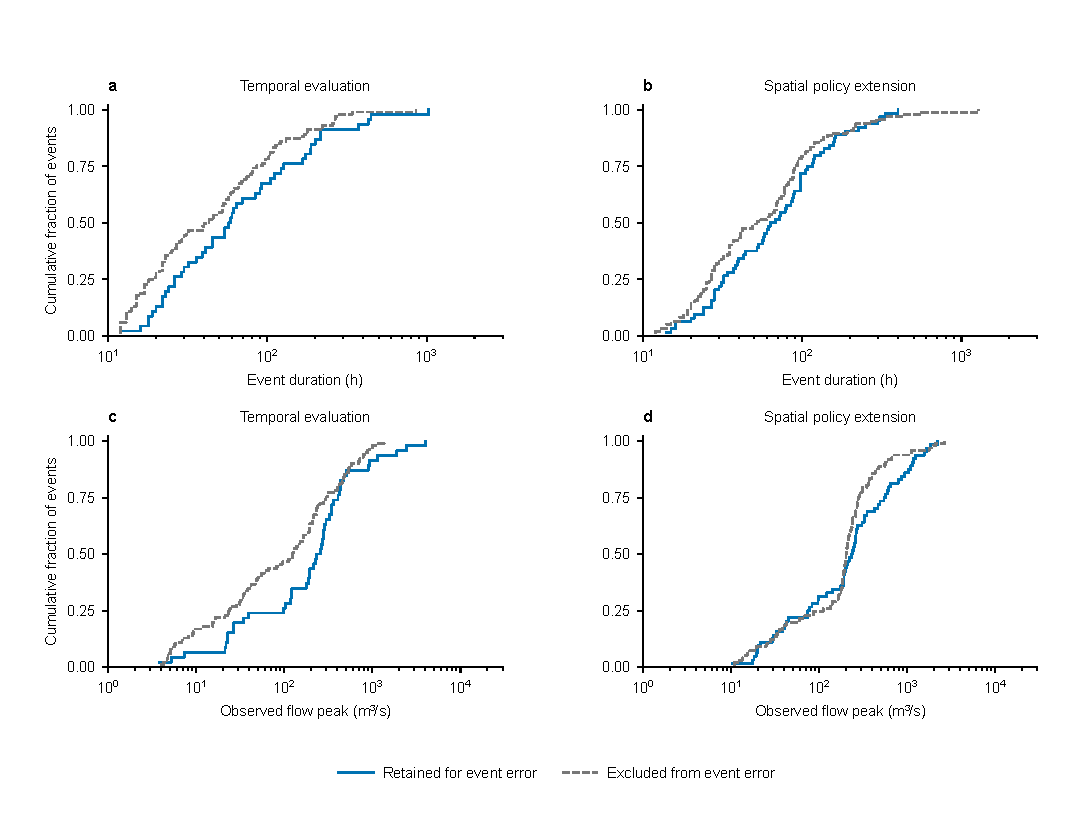
\includegraphics[width=\textwidth]{figures/FigS1.pdf}
\end{center}

\noindent\textbf{Fig. S1} Detected events retained in and excluded from the event error evaluation. Empirical cumulative distributions compare event duration (a, b) and observed peak flow (c, d), and each distribution is normalised by its own event count, which is 46 retained and 101 excluded events for the temporal cohort and 64 retained and 97 excluded events for the spatial cohort. Events are nested within sites. Retention combines reference hour coverage, observable flow boundaries and positive reference load, and exclusion does not necessarily mean a missing concentration at every hour. Peak flow distributions reflect the station mix as well as event hydrology, and they do not establish that missingness is confined to small events. The common logarithmic x axis limits are held equal across cohorts, and no significance test or missing load imputation is performed.

\begin{center}
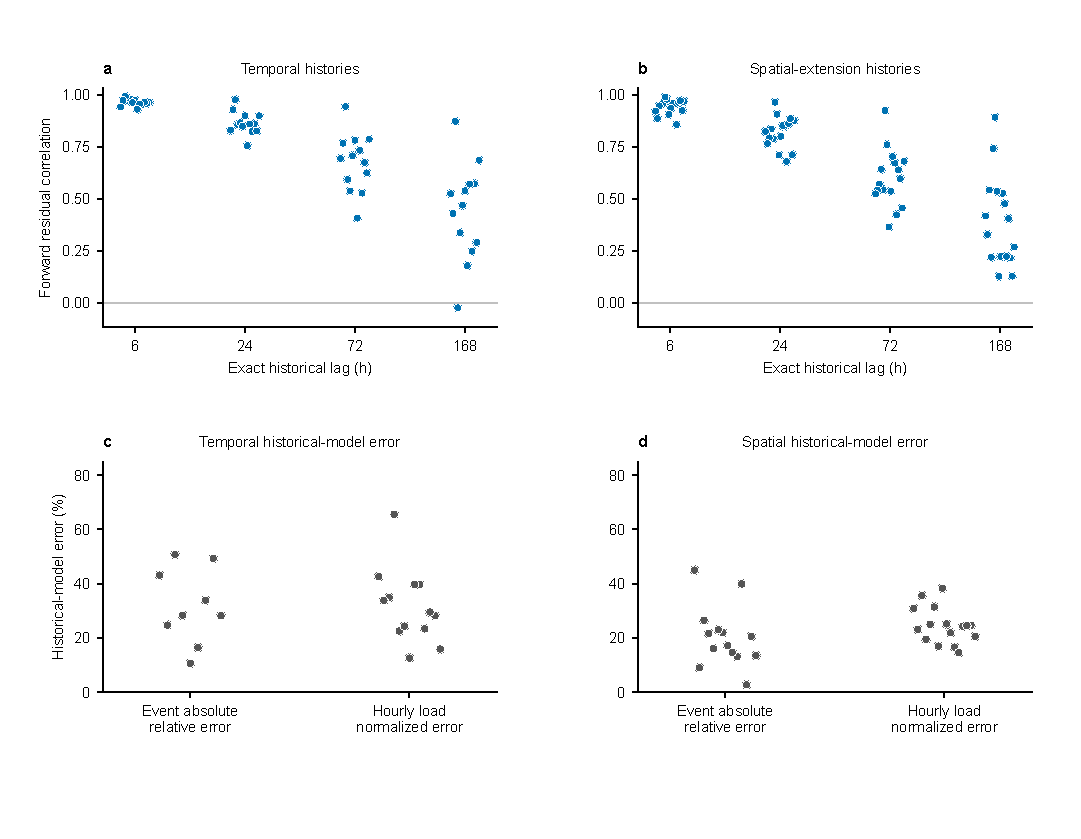
\includegraphics[width=\textwidth]{figures/FigS2.pdf}
\end{center}

\noindent\textbf{Fig. S2} Historical residual persistence and the need for concentration feedback vary across station years. (a, b) Each point is a historical calibration year residual correlation from a forward model trained only on earlier permitted years, for one data eligible target station year. A pair at a lag of 6, 24, 72 or 168 h requires qualified labels at both endpoints and throughout the intervening interval, and exact pair counts accompany the source table. These correlations describe persistence and they do not identify an optimal correction memory constant. (c, d) Errors of the historical model with no new concentration labels, averaged over model seeds within station year. Event error is the mean absolute relative error across retained events, and hourly normalised error is summed absolute load error divided by observed reference load. Rows with undefined event error are not drawn, and hourly error points retain all data eligible station years. Points, years and seeds are not independent rivers, and these are descriptive context diagnostics rather than a fitted relationship between persistence and policy benefit.

\begin{center}
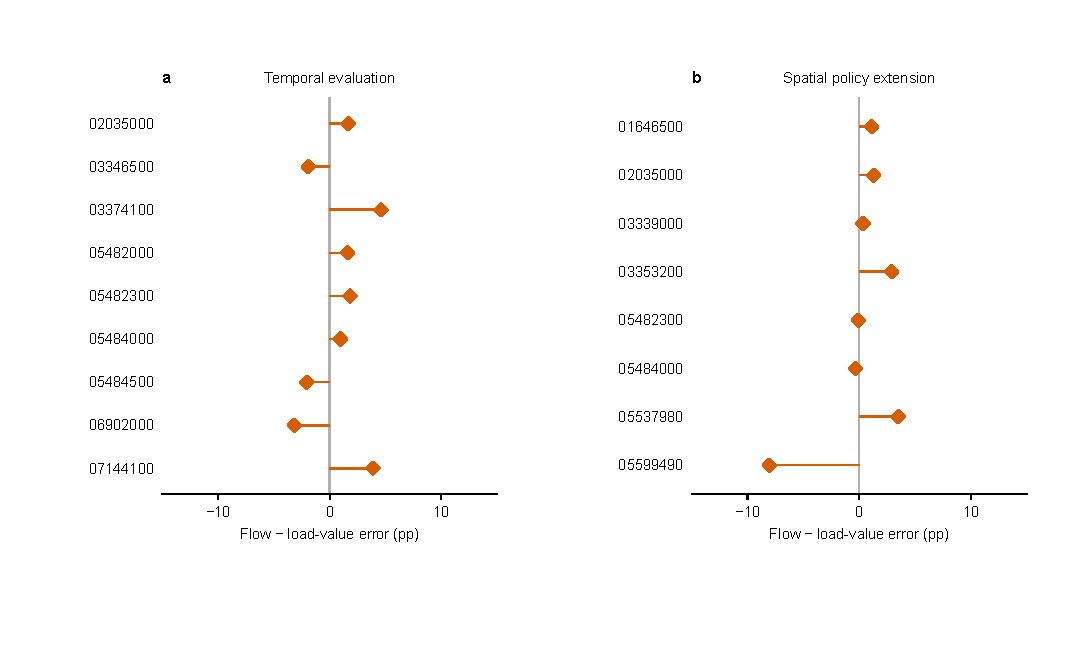
\includegraphics[width=\textwidth]{figures/FigS3.pdf}
\end{center}

\noindent\textbf{Fig. S3} Station specific flow trigger minus load value event error at 96 attempted samples per year and a 24 h actual delay, using the same latest residual reconstruction. Positive values favour load value, and all event eligible sites appear in station number order including negative differences. Site specific uncertainty intervals are not inferred from seed replication, and for the spatial extension years and seeds are averaged within site. These are percentage point differences in relative event error rather than absolute load improvements.

\begin{center}
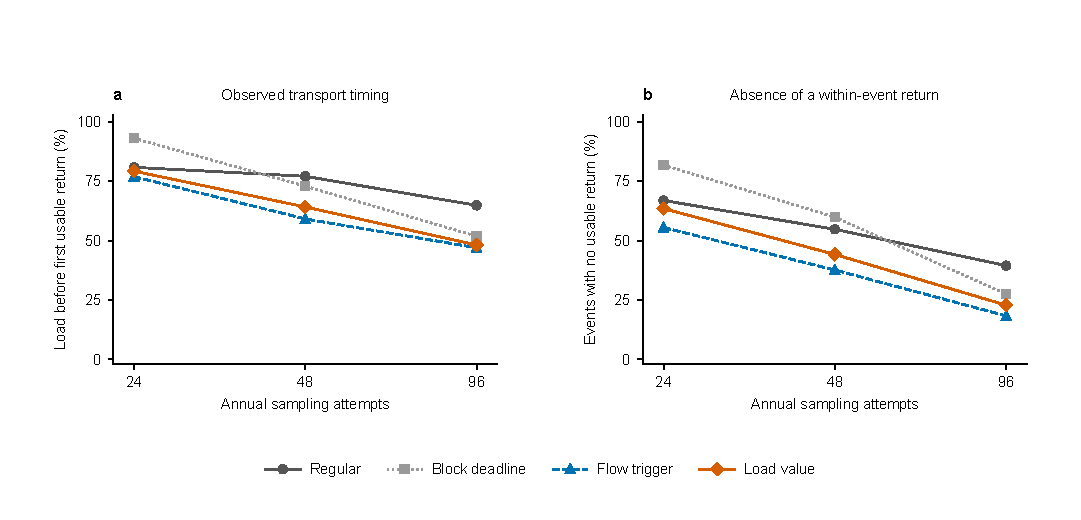
\includegraphics[width=\textwidth]{figures/FigS4.pdf}
\end{center}

\noindent\textbf{Fig. S4} Actual concentration return timing under the temporal replay with a 24 h result return delay. (a) Fraction of observed event reference load transported before the first usable return within the event, where a returned result may originate from a sample collected before onset. When no usable result returns within an event the fraction is set to one, and an earlier returned result can still inform prediction. (b) Fraction of events with no usable return within the event. Both summaries average seeds within each of the 46 physical events, then events within station year, then years within site, and then the nine event eligible sites with equal weight, so three seed replays are not treated as independent events. These are descriptive timing measures rather than the fixed onset windows of Fig. 2, measures of successful correction or error lower bounds, and the ordinate in (a) is not the load weighted total of the cohort.

\begin{center}
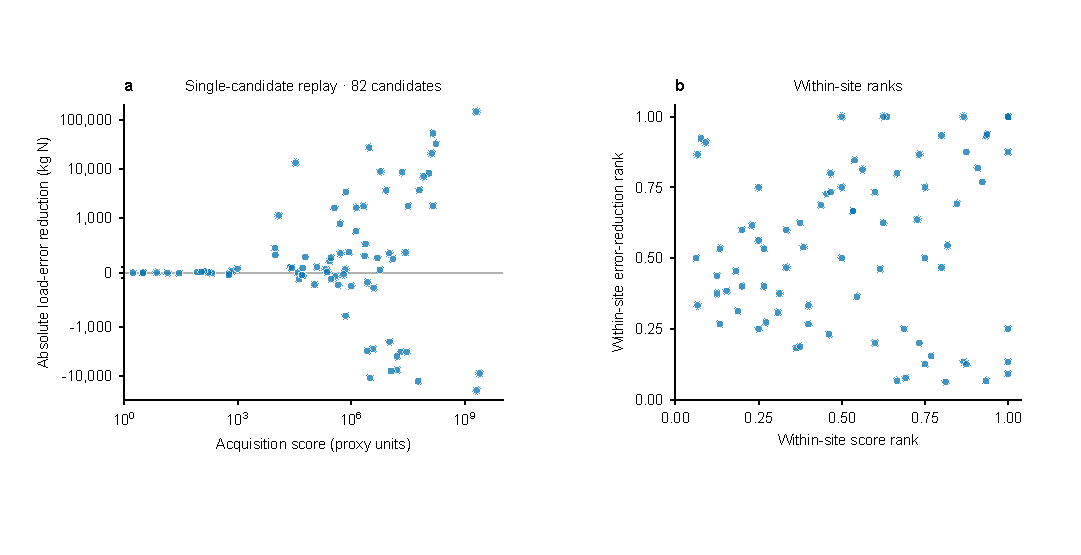
\includegraphics[width=\textwidth]{figures/FigS5.pdf}
\end{center}

\noindent\textbf{Fig. S5} The acquisition score is a proxy rather than an observed utility estimate. (a) A candidate diagnostic adds one sample to an otherwise fixed replay and compares absolute accumulated load error over its diagnostic window, where positive kilogram differences mean less absolute load error after the added result and negative differences mean more. Of 168 planned candidates, 82 qualified for the diagnostic, 50 beneficial and 32 harmful, spanning seven sites. The raw score uses a logarithmic x axis, and the signed error reduction uses a symmetric logarithmic y axis that is linear within $\pm$1,000 kg N so that negative outcomes and the large positive outcome remain visible. (b) Fractional ranks computed within site from the supplied diagnostic table, where tied or identical ranks may overlap. No fit, significance test, subgroup search or causal claim is added, and the window level added sample contrast is not the effect of deploying an altered closed loop policy. Eligibility requires spacing, a usable concentration and the specified window reference coverage, which limits the diagnostic population, and absolute kilogram improvements and relative event error improvements remain distinct outcomes.

\bibliography{sn-bibliography}

\end{document}